\chapter{Numerical Experiments}
\label{chapter:NumericalExperiments}

\section{Cantilever Beam}
\subsection{Problem Description}
% Youns modulus 1,000,000
% poisson = 0.3
% density = 0.001
% units?

% newton load steps
% setup of beam pictures
% discretization strategy (maybe table of values?)
% tartaros setup variables
% \begin{figure}[hbt]
%     \centering
% \begin{circuitikz}
%     %wall
%     \fill[pattern=north east lines] (0,.5) rectangle (0.25,4);
%     \draw (0.25,.5) -- (0.25,4);
%     % beam
%     \draw[fill=gray!40] (0.25,2) rectangle (6,2.5);
%     % length of beam
%     \draw[<->|] (0.25,1.8) -- (6,1.8) node[midway,below] {$L$};
%     % force
%     \draw[->] (6,4) -- (6,2.5) node[midway,left] {$F$};
%     \draw[dashed] (6,2.5) -- (9,2.5);
%     \draw[dashed] (6,2) -- (9,2);
%     \draw[fill=gray!40] (9,2) rectangle (10,2.5);
%     \draw[] (9,1.8) -- (10,1.8) node[midway,below] {$w$};
%     \draw[|<->|] (10.2,2) -- (10.2,2.5) node[midway,right] {$h$};
% \end{circuitikz}
% \end{figure}

To compare the performance of a Krylov solver preconditioned with SA-AMG with that of a direct solver, a scaling study was performed on two different 3 dimensional cantilever beams of varying height $h$. The factor $r$, chosen to be 10 and 100, determined the ratio of length-to-height. The beam material was a Neo-Hooke material with a Young's modulus of $E = 10\ \text{MPa}$ and a Poisson's ratio of $\nu = 0.3$. The beam shown in Figure~\ref{fig:beam} is fixed with Dirichlet boundary conditions on one end and has a Neumann load on the other end. The beams were discretized with varying amounts of elements in increments of 10,000 for one study and 1,000,000 for another. For the discretization elements, the condition was imposed that the element aspect ratio remain as close to 1 as possible, such that the elements were cube-shaped. The finite elements were chosen to be solid HEX8 elements.

% machine setup

\begin{figure}[h]
    \centering
    \begin{tikzpicture}
    
    % \draw[->] (0,0,0)-- node[pos=.7,below] {x} ++(6,0,0);
    % \draw[->] (0,0,0)--++(0,3,0) node[pos=.75, left=7mm,rotate=90]{y};
    % \draw[->] (0,0,0)--++(0,0,4) node[midway, sloped, above] {z};
    % \fill (10,0.1,1) circle(3pt);
    \draw[pattern=north west lines] (0,1,1.5)--(0,-0.5,1.5)--(0,-0.5,-1)--(0,1,-1)--cycle;

    \draw[fill=gray!40] (10,0.5,1)--(10,0.5,0)--(0,0.5,0)--(0,0.5,1)--cycle;
    \draw[fill=gray!40] (10,0.5,1)--(10,0,1)--(10,0,0)--(10,0.5,0);
    \draw[fill=gray!40] (10,0,1)--(0,0,1)--(0,0.5,1)--(10,0.5,1) -- cycle;

    \draw[dim] (0,-0.75,1.2) -- (10, -0.75, 1.2) node[midway, below] {$L = 10$ m};
    \draw (0, -0.5, 1) -- (0, -0.9, 1.2);
    \draw (10, -0.5, 1) -- (10, -0.9, 1.2);
    \draw[dim] (10,-0.5,0.5) -- (10, -0.5, -0.5) node[midway, below, xshift=0.7cm] {$w = 1$ m};
    \draw (10, -0.4, 0.6) -- (10, -0.6, 0.4);
    \draw (10, -0.4, -0.4) -- (10, -0.6, -0.6);
    \draw[dim] (10.5, 0, 0) -- (10.5, 0.5, 0) node[midway, right] {$h = L/r$};
    \draw (10.4, 0, 0) -- (10.6, 0, 0);
    \draw (10.4, 0.5, 0) -- (10.6, 0.5, 0);
    \draw (10.0, 0.5, 0) -- ++(0, 0, 1.0) node[midway, above, yshift=0.4 cm] {$F = \frac{1}{(r/10)^3}$ N};
    \foreach \z in {0,0.25,...,1} {
        \draw[-latex] (10.0,0.5,\z) -- ++(0,-0.5,0);
    }

    % \fill[pattern=north east lines] (0,.5,0) rectangle (0.5,0.25,1);

\end{tikzpicture}
\caption{3 dimensional cantilever beam}
\label{fig:beam}
\end{figure}

% describe the solver setup
The solver consists of a nonlinear Newton solver performing a time integration scheme, although the problem being considered is non-transient. At each Newton iteration, a linear system of equations has to be solved. The load $F$ starting at 0 is increased by a constant amount each time step so that it reaches the desired load value at the final time step. This is done to give the Newton statics solver better convergence properties, since the incrementally applied load results in the solution being within the method's radius of convergence. For this experiment, 10 load steps were used, and the statics solver was considered converged if the residuals for the Newton iterations were below $10^{-5}$.

Within each Newton iteration, the system of equations is solved with a GMRES method that is preconditioned with an SA-AMG solver. The GMRES convergence criterion of $\norm{r_k}_2/\norm{r_0}_2 < 10^{-6}$ was used, with a maximum number of iterations of 1000. The particular implementation was a restarted GMRES which would restart after the Krylov subspace reached a chosen size of 100.

\begin{table}[ht]
    \centering
    \begin{tabular}{|l|l|} 
    \hline
    Setting Name & Value \\
    \hline
    Cycle Type                          & V                     \\
    Max Levels                          & 7                     \\
    Muelu Reuse Strategy                & Nothing               \\
    PDE Equations                       & 3                     \\
    \hline
    Aggregation: Type                    & Uncoupled             \\
    Aggregation: Damping Factor          & 1.33                  \\
    Aggregation: Nodes Per Aggregate    & 27                    \\
    \hline
    Smoother: Sweeps                     & 1                     \\
    Smoother: Damping Factor             & 1                     \\
    Smoother: Pre- or Post-Smoothing     & Both                  \\
    Smoother: Type                       & Chebyshev             \\
    Chebyshev Degree (Fine to Coarse)       & 12, 6, 6, 6, 6, 6, 1  \\
    Eigen-Analysis: Type                 & CG                    \\
    Eigen-Analysis: Iterations           & 10                    \\
    \hline
    Coarse-Level: Solver                 & Amesos-UMFPACK        \\
    Coarse-Level: Max Size               & 20000                 \\
    Coarse-Level: Pre- or Post-Smoothing & Pre                   \\
    Coarse-Level: Sweeps                 & 1                     \\
    Coarse-Level: Split Communicator     & False                 \\ 
    \hline
    Repartitioning                      & Enabled               \\
    Repartitioner                       & ParMETIS              \\
    Repartitioning: Max-Min Ratio       & 1.2                   \\
    Repartitioning: Min per Proc        & 1000                  \\
    \hline
    \end{tabular}
    \caption{MueLu Settings used for various numerical experiments}
    \label{table:muelu}
\end{table}

The SA-AMG preconditioner was set up with the MueLu settings from Table~\ref{table:muelu}. The maximum amount of level was limited to 7, and a coarse level size of 20000 DOFs was used in order to limit the amount of coarsening.

The Chebyshev polynomial smoother was used, since the computational kernel involves a matrix-vector product which works well for SPD matrices. This smoother requires estimates of minimum and maximum eigenvalues of $A$, and recursively forms Chebyshev polynomials of increasing degree which are used to form the residual. The full method is detailed in Gutknecht et al.~\cite{Gutknecht2002}. The degree of the polynomial is reduced at coarser levels to reduce the amount of computation. At the coarsest level, the problem is solved with the UMFPACK solver from the Amesos library, which is a direct sparse LU factorization method~\cite{Davis2004}.

The uncoupled aggregation strategy is used, which avoids aggregating nodes which are assigned to different processors. This aggregation method has the advantage of reducing communication between processors during aggregation as well as prolongator smoothing, but can result in some aggregates near processor boundaries being too small. Since aggregates cannot cross processor boundaries, the coarse level problem might have too many nonzeroes per row. Additionally, some processors could have more work than others on the coarse level, which results in other processors having to wait (\cite{Tuminaro2000}, ~\cite{Hu2014}). The number of nodes per aggregate was chosen to be 27 for the 3D problem, since aggregates having a diameter of less than three can lead to high iteration costs~\cite{Tuminaro2000}.

With the uncoupled aggregation process, rebalancing the problem among the processors is necessary. This is implemented with the ParMETIS library, and reduces the number of processors on coarse levels such that a minimum amount of DOFs of 1000 per processor is achieved. The problem is also rebalanced if any processor has more than 1.2 times the amount of nonzeroes as another processor.

\subsection{Results}
The simulations were run with up to 40 cores on 4 Intel Xeon Silver 4114 processors. The
% NOTE: 5,997 is the \columnwidth in inches (for matplotlib)
%       Font is 10.91 pt captions
% \begin{figure}
%     \includegraphics[width=\columnwidth]{test.pdf}
%     \caption{This is a placeholder to measure the width of a plot. Its with is set to \texttt{columnwidth}.}
% \end{figure}

% example pic of rebalancing domain
% strong vs weak scaling
% amdahl's law
% why not perfect scaling? communication
% gmres iterations, timing, operator complexity? gee2009 eqn (18)
% comparison to superlu

% side-by-side example
% \begin{figure}[h]
%     \centering
% \begin{subfigure}{0.45\columnwidth}
%     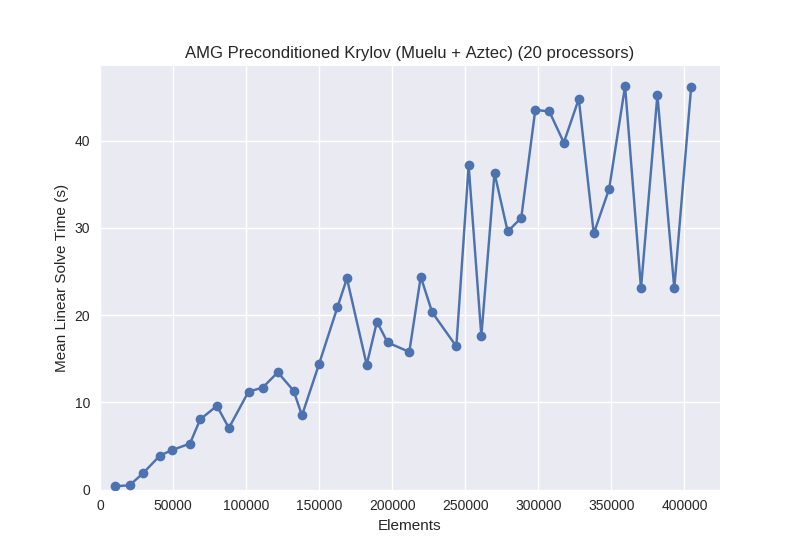
\includegraphics[width=\textwidth]{beam/muelu_beam_scaling.pdf}
%     \caption{}
% \end{subfigure}
% \begin{subfigure}{0.45\columnwidth}
%     \includegraphics[width=\textwidth]{beam/muelu_gmres_iters.pdf}
%     \caption{}
%     \label{fig:1}
% \end{subfigure}
% \end{figure}

\begin{figure}[ht]
\begin{subfigure}{\columnwidth}
    \centering
    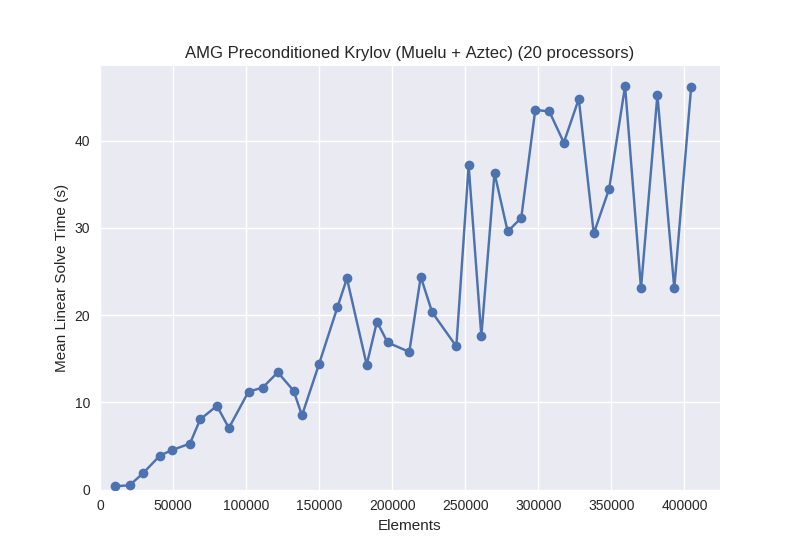
\includegraphics[width=\columnwidth]{beam/muelu_beam_scaling.pdf}
    \caption{Mean linear solve time per Newton iteration (20 Newton iterations and 10 load steps total).}
    \label{fig:3}
\end{subfigure}
\begin{subfigure}{\columnwidth}
    \centering
    \includegraphics[width=\columnwidth]{beam/muelu_gmres_iters.pdf}
    \caption{Mean GMRES iterations per Newton iteration (20 Newton iterations and 10 load steps total).}
    \label{fig:4}
\end{subfigure}
\caption{Weak scaling results (\texttildelow10,000 elements per processor) for the cantilever beam example. Comparison of results for different beam length-to-height ratios $r$. A larger $r$-value is more slender.}
\end{figure}

\begin{figure}[ht]
    \begin{subfigure}{\columnwidth}
        \centering
        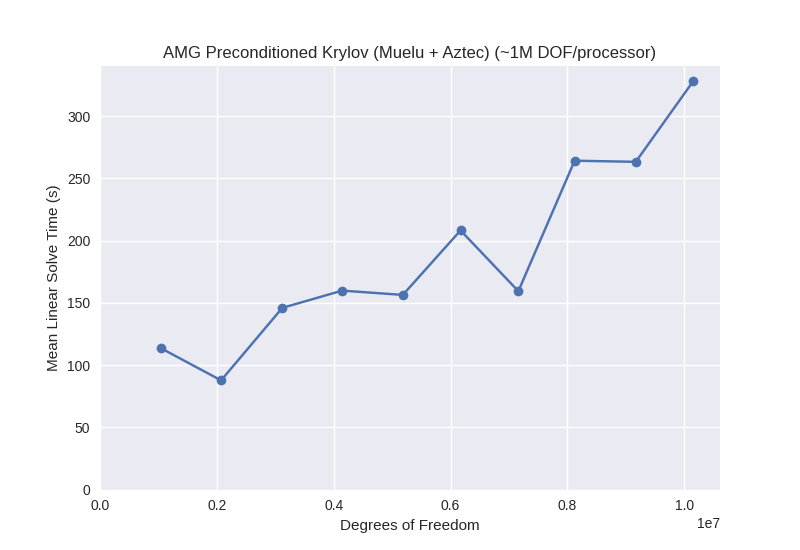
\includegraphics[width=\columnwidth]{beam_10M/muelu_ratio_10_beam_scaling.pdf}
        \caption{Mean linear solve time per Newton iteration (20 Newton iterations and 10 load steps total).}
        \label{fig:3}
    \end{subfigure}
    \begin{subfigure}{\columnwidth}
        \centering
        \includegraphics[width=\columnwidth]{beam_10M/muelu_ratio_10_gmres_iters.pdf}
        \caption{Mean GMRES iterations per Newton iteration (20 Newton iterations and 10 load steps total).}
        \label{fig:4}
    \end{subfigure}
    \caption{Weak scaling results (\texttildelow1,000,000 elements per processor) for the cantilever beam example using $r = 10$.}
\end{figure}

\begin{figure}[ht]
    \centering
    \includegraphics[width=\columnwidth]{beam/ratio_10_prec_beam_scaling.pdf}
    \caption{Solve time comparison of SuperLU direct solver against Aztec GMRES preconditioned with MueLu SA-AMG. Note the scaling is represented on a log-scale.}
    \label{fig:5}
\end{figure}

\section{Turbojet Engine Blade}
\subsection{Problem Description}
% discussion of nullspace vectors, form for 3D elasticity
% stand-alone solver, only A was available

\subsection{Results}
% graphs, what was tried

\section{Cylindrical Shell}
\subsection{Problem Description}
% diagram of shell, properties used
% different height ratios, increasing force until snap through

% citing the same stuff from bischoff dissertation
% citing paper on shell stuff

\subsection{Results}

% graph/table of forces required for snap-through
%